\subsection{Breakers}
\subsubsection{Breaker Overview}
The breaker system is half of the smart breakers system aimed at providing the consumer with better circuit protection in addition to circuit information. 

In addition to allowing for a safer installation, using solid state technology improves safety through faster response time. Accuracy can also be improved since the control logic for the switch is much easier to calibrate than an induction coil which is what breakers currently use. Cost of a smart breaker is higher because of the added switching feature, but the team decided that it was acceptable because of the benefits of having a safer system and improved functionality.

\subsubsection{Breaker System Diagram}
\begin{figure}[htbp]
\begin{center}
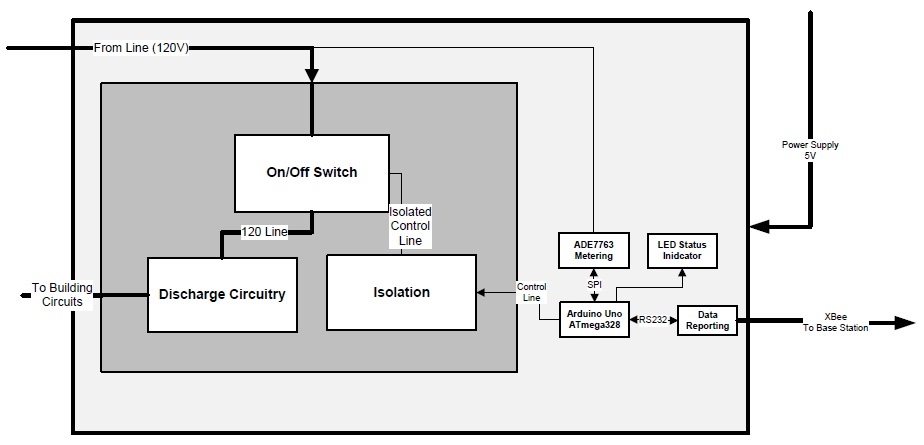
\includegraphics[width=6in]{includes/NJSmartBreakerSwitch}
\caption{Block diagram highlighting the breaker components}
\label{fig:breaker_block_diagram}
\end{center}
\end{figure}

The diagram above shows the breaker technology within the outlined box in relation to the other aspects of the smart breaker. For the design of the switching part of the breakers, the isolating circuit, the discharge circuitry and on/off switch are the three key components needed for a safe and fully functional breaker system. The controls and monitoring are also important for a fully working system, but the team decided those functions were better handled by the monitoring part of the smart breakers.

\subsubsection{Component Selection}
On/Off Switch

The team focused initially on selecting an appropriate switching component and looked at SCRs, triacs, FETs, thyristors and solid state relays as possible options based on their ability to work well with high voltage and current levels. The table below shows a few additional benefits and drawbacks of each.

\begin{figure}[htbp]
\begin{center}
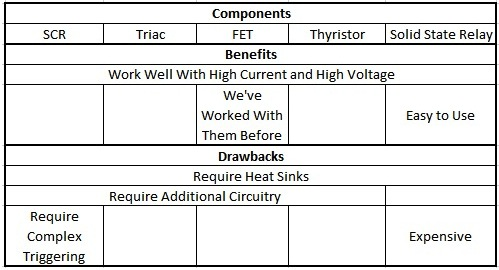
\includegraphics[width=5in]{includes/NJSwitchComponentOptions}
\caption{Table comparing switching components}
\label{fig:switch_component_options}  
\end{center}
\end{figure}

Each of the options does require the use of heat sinks, which is not ideal for a final design because it is difficult to dissipate heat from inside a standard breaker box. This one of the first parts of the design that would need to change for the transistion from proof of concept to final product to happen. Ultimately, the team decided to use solid state relays, due to their ease of use for the designer and lack of need for additional circuitry, which would require significantly more time for parts to arrive and for assembly. While solid state relays may not be optimal for a final design, the team decided to spend more time working on the primary goal of measuring power. More testing needs to be completed to determine what the efficiency of the switch is since any additional power used by the system has to be subtracted from the total saved. 

Isolation Circuit

The isolation circuitry's purpose is to protect the control logic should any line voltage cross over to the control side. The team selected an opto isolator for this purpose based on availability, ease of use, and functionality. 

In the prototype design, the functionality of the isolation is somewhat compromised since it uses only a single power source. However, since the breakers were primarily a proof of concept, the team decided it was acceptable to spend more time on other areas of the project instead of physically building the second power supply needed for a final design.   

Discharge Circuitry

At high currents and voltages, suddenly turning the circuit off can cause damaging transients. The discharge circuitry captures those transients before they become a problem and dissipates them later in a safe manner. In a final design, energy storing components, primairly capacitors or inductors, would be used to quickly absorb the transients before discharging them at a much slower rate. The team did not include this aspect in the prototype since it is not critical to demonstrating the smart breakers' ability to read power.

\subsubsection{Testing}
Following selection of the switching component, the team ran a few basic tests and found that at low current levels the solid state relay functions as well as standard air-gap breakers. The comparison to standard air-gap breakers was measured by visually watching for transients using an oscilloscope while turning the relay and breaker on and off. 

With loads between $150 \ohm$ and $1.5\kilo\ohm$ attached to the relay, the turn on voltage remained constant at 2.8 V. This was determined by increasing the control voltage until the load circuit turned on. Similarly, the turn off voltage was tested by lowering the control voltage until the load circuit turned off, and again within the range of loads attached, the turn off voltage stayed constant at 2.8 V. Although the team hoped to design for currents up to 20 A, the ability to switch currents higher than 1 A was not tested, primarily because the discharge circuitry had not been developed. After implementing the discharge circuitry, the same test would be done, except with loads that require much higher current. The microcontroller would also have to have a new threshold value programmed, but this will not affect how the hardware works.

\subsubsection{Future Work}
Solid state relays work well to demonstrate the smart breakers' ability to monitor and control electrical power, but are not a good selection for a consumer device because of high cost and need for heat sinks. Given more time, the team would like to design breakers that make use of another switching component that would be selected based more on cost and minimizing the need for heat sinks instead of easy use in a design. Adding discharge circuitry is another aspect the team would like to include. 
